\section{2050 Energistrategi}

Den danske regering har skrevet under på, at Danmark i 2050 skal være fuldstændig uafhængig af fossile brændsler. Det vil sige at Danmark skal være fri for kul, olie og naturgas. Dette medfører at Danmark fremadrettet skal satse på bæredygtig energiteknik, herunder vindenergi, bølgekraft, solceller og biomasse. I 2020 skal $42 \%$ af Danmarks energiproduktion komme fra vindenergi, som set på figur \ref{fig:Cirkel}.

\begin{figure}[H]
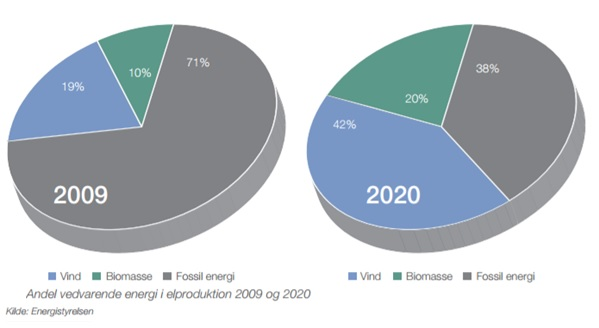
\includegraphics[scale=0.85]{Billeder/Cirkeldiagram_probana}
\caption{Cirkeldiagram over Danmarks energiproduktion}
\label{fig:Cirkel}
\end{figure}

\begin{figure}[H]
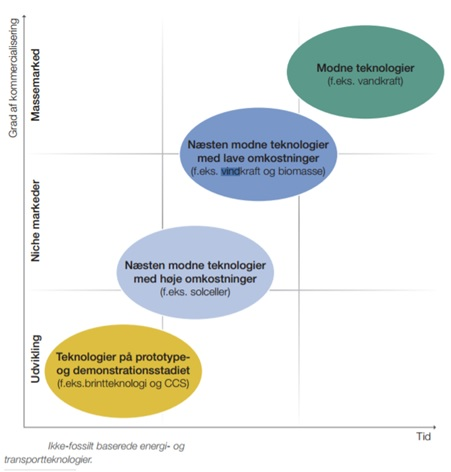
\includegraphics[scale=0.85]{Billeder/Baeredygtige_energiiniti}
\caption{Grad af kommercialisering i energisektoren på verdensplan}
\label{fig:Massemarked}
\end{figure}
Vi kan se på figur \ref{fig:Massemarked} at vand-, vindkraft og biomasse allerede er i massemarked, så det er allerede muligheder, som bliver brugt og videreudviklet. Imens solceller bliver solgt og forbedret løbende. Brintteknologi er stadig i udviklingsfasen.
I Danmark er vindenergien i højsædet, grundet vores kystnære områder, samt flade landskab.